\subsubsection{16.01.15}
\begin{enumerate}
	
	\item Время начала и окончания собрания: 16:30 - 21:30.
	
	\item Цели собрания: 
	\begin{enumerate}
		
		\item Потренироваться в управлении роботом.
		
		\item Выявить недостатки конструкции или программы в ходе тренировок.
		
	\end{enumerate}

	\item Проделанная работа:
	\begin{enumerate}
		
		\item Сегодня мы тренировались в управлении роботом. Программа управления движением робота работала безупречно; подъемник раздвигался плавно, Желоб и направляющая для шаров обеспечивали точность забрасывания мячей в корзину. На данный момент на то, чтобы захваатить 3 больших мяча (у нас в распоряжении их всего 3) и забросить их в корзину (ее роль выполняет водосточная труба из ПВХ диаметром 11 см и высотой 90 см) нам требуется от 30 до 60 секунд, но в настоящей игре мы планируем возить корзину за собой, так что мы не будем тратить время на подъезд к корзине. С помощью тренировок мы планируем сократить время сбора одной порции мячей (5 шт.) до 30 и менее секунд.
		
		\item Поскольку в ходе тренировок обнаружилось, что некоторые мячи выбрасывает вбок, мы решили поставить дополнительные откосы, направляющие мячи в ковш.
		\begin{figure}[H]
			\begin{minipage}[h]{0.2\linewidth}
				\center  
			\end{minipage}
			\begin{minipage}[h]{0.6\linewidth}
				\center{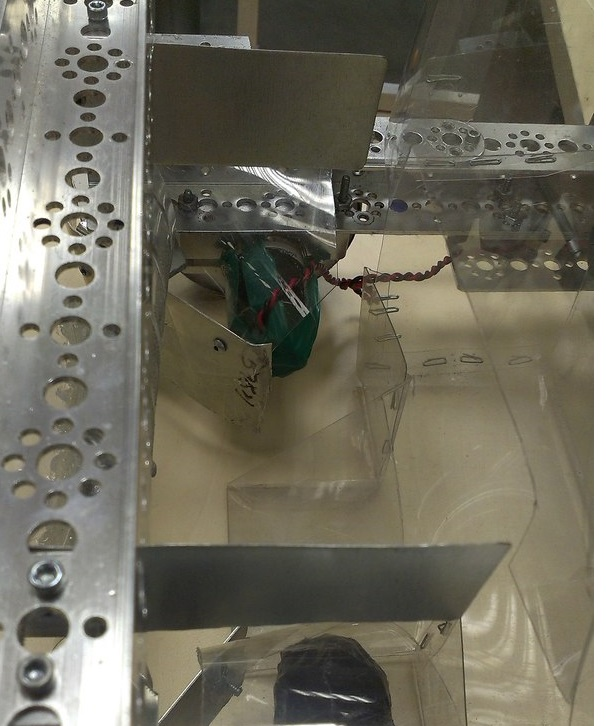
\includegraphics[scale=0.2]{days/16.01.15/images/01}}
				\caption{Дополнительные откосы}
			\end{minipage}
		\end{figure}
		
        \item Поскольку основная работа над механической частью робота завершена, а программа управляемого периода написана, настало время совершенствовать программу автономного периода. Сегодня было предложено несколько версий автономного периода:
        \begin{enumerate}
        	
        	\item Съехать с пандуса, забросить маленький мяч в подвижную корзину высотой 60 см. С помощью ИК-датчика найти корзину 120 см и забросить в нее большой мяч. Заехать в зону. (Максимум 130 очков)
        	
        	\item Съехать с пандуса, забросить маленький мяч в подвижную корзину высотой 60 см и захватить ее. Отвезти корзину 60 см в зону и вернуться за корзиной 90 см. Захватить ее и забросить в нее большой мяч. Завезти корзину 90 см в зону. (Максимум 140 очков)
        	
        	\item Съехать с пандуса, забросить маленький мяч в подвижную корзину высотой 60 см и захватить ее. С помощью дополнительного захвата корзин захватить корзину 90 см. Привезти обе корзины в зону. Отпустить корзину 60 см, подъехать ближе к корзине 90 см и забросить в нее большой мяч. Заехать в зону. (Максимум 140 очков)
        	
        \end{enumerate}

	\end{enumerate}
	
	\item Итоги собрания:
	\begin{enumerate}
		
		\item Мы попрактиковались в управлении роботом.
		
		\item Система захвата мячей доработана.
		
		\item Были разработаны стратегии автономного периода.
		
	\end{enumerate}
	
	\item Задачи для последующих собраний:
	\begin{enumerate}
		
		\item Продолжать тренироваться.
		
		\item Усовершенствовать автономный период.
			
	\end{enumerate}
\end{enumerate}
\fillpage
